Among the definitions one gives of \textbf{Machine learning} we can say that it is a \textit{"Field of study that gives computers the ability to learn without being explicitly programmed"}. Nowadays, the \textit{Artificial intelligence} is in general that the electricity was in the 19$^\text{th}$ century. Something of paramount importance! \\
There are several methodologies and subfields in Machine Learning and the distinction is based on \textit{how much and how} the human collaborate and of the type of provided data. The most important classification is the one between:
\begin{itemize}
    \itemsep-0.3em
    \item \textit{Supervised learning} (this course), is the approach which uses \textbf{a-priori knowledge} embedded in the data that are used for training algorithms and recognize patterns;
    \item \textit{Unsupervided learning}, is the approach at the opposite whose main feature is not using \textit{labeled data} for assess the tasks.
    \item \textit{Other approaches}. Due to its vastness, in machine learning you can find for sure other subfields. For example the \textit{Reinforcement learning, Semi-Supervised learning, trasnfer learning}. However they are all outside the purposes of this course. 
\end{itemize}

\begin{figure}[h]
    \centering
    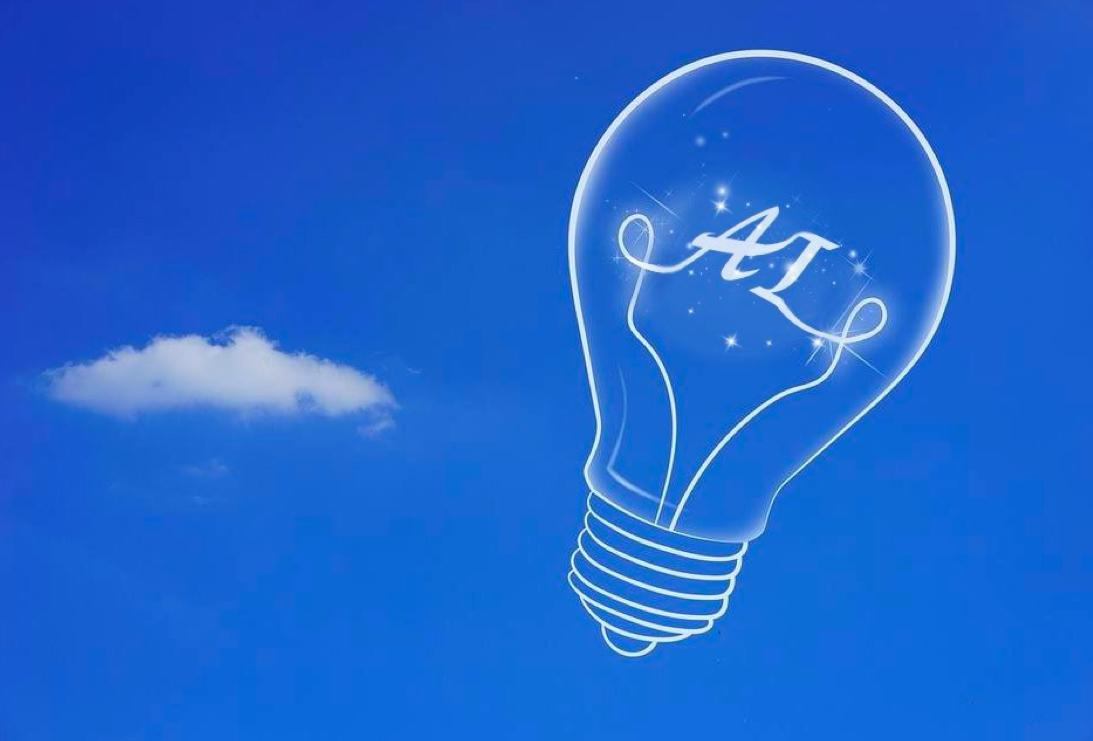
\includegraphics[scale=0.2]{img/AI.jpeg}
\end{figure}

\section{Supervised learning}
From \textsc{Wikipedia (EN)}: \textsf{Supervised learning (SL) is a paradigm in machine learning where input objects (for example, a vector of predictor variables) and a desired output value (also known as a human-labeled supervisory signal) train a model.} In the following we are giving some simple introductory examples about two among the most used techniques in supervised learning.
\subsection{Linear Regression}
Let us imagine we are supposed to create a model that allows us to \textbf{predict the price of an house}. For sake of simplicity and clarity, suppose that our \textit{dataset entries} have one feature (the house size in ft$^2$) and the \textit{price} which represents the \textbf{correct answers}.
Using this data we seek for a model which could predict, given the size of an unknown house, his price (in dollars, \$). Several choices can be made. At first, using either a linear or a nonlinear model and so on. It is remarkable that -- even in such a simple example -- we are facing a \textbf{supervised} problem since the right answers are given! This particular case is a problem of \textbf{regression} since we want to \textbf{predict a continuous valued output}, in our case the price.

\begin{figure}[h]
    \centering
    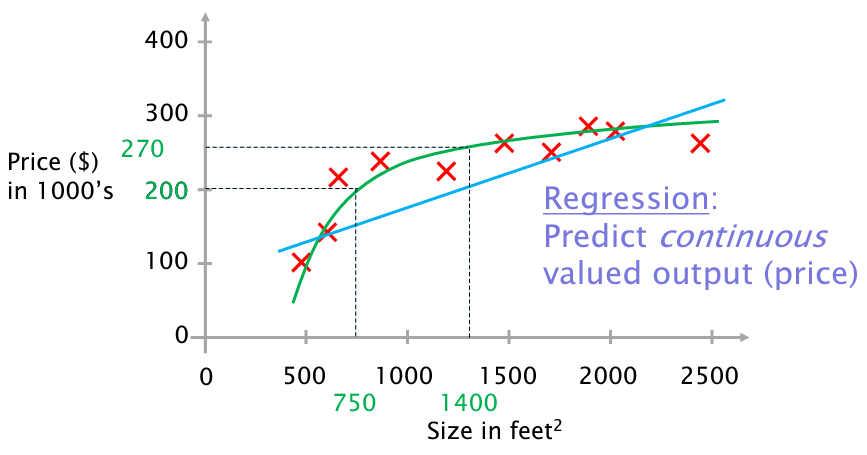
\includegraphics[scale=0.5]{img/prices.png}
\end{figure}

In the figure above is shown the example in which two different models are used, clearly the predicted values for an unknown record is different according to the chosen model.

\subsection{Classification}
On the other hand, when we want to predict a discrete value (eg. YES/NO), we have a \textbf{classification} problem. Again, let us consider a trivial example: we want to predict whether a tumor is malignant or not according to its size. Even in this case we have one feature for the data (\textit{tumor size}) and all the training data are labeled with the YES/NO answer.

\begin{figure}[h]
    \centering
    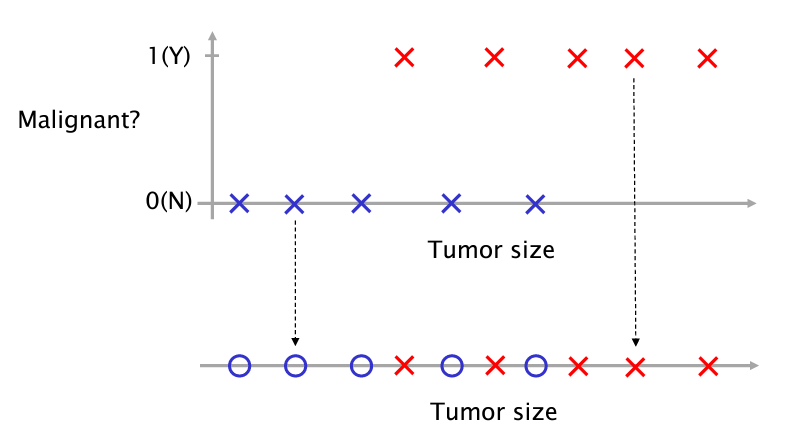
\includegraphics[scale=0.5]{img/tumor.png}
\end{figure}

The figure shows a graphical representation of the dataset. In this case since the answers are associated with different symbols, a more compact representation is given by a one-axis diagram: one feature is given, furthermore a different symbol is associated to different classes. Note that in this case we are in front of a a \textbf{binary classification problem}, in general the classes to predict are not necessarily in number of two. \\
This was just an example to understand and introduce the problem, but in real-world applications, one feature is not sufficient to build a good model! For sake of clarity, let us complicate a little bit the example we have just presented by adding a new feature associated with the \textit{age of the patient}.

\begin{figure}[h]
    \centering
    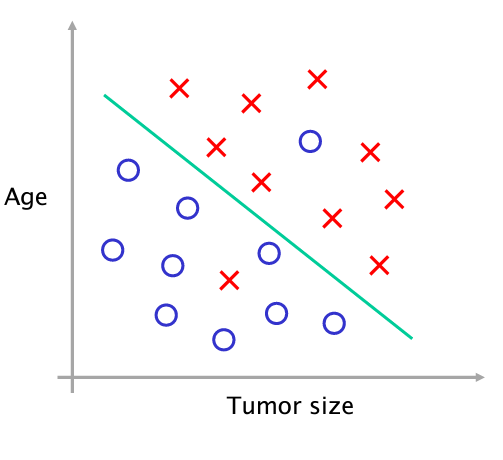
\includegraphics[scale=0.5]{img/tumor_more.png}
    \caption{Bi-variate problem with linear decision boundary}
\end{figure}

In this case the data set is represented in a 2D graph, one axis for each feature and a different symbol for each class. Now, given a record associated with a new patient, what is the class for its tumor? In this case can be useful to individuate a \textbf{decision boundary} according to which one can decide clearly what is the prediction (Positive/Negative). In the two parts there are some outliers, for this reason one can be tempted to build a more "accurate" decision boundary that perfectly split the two classes.

\begin{figure}[h]
    \centering
    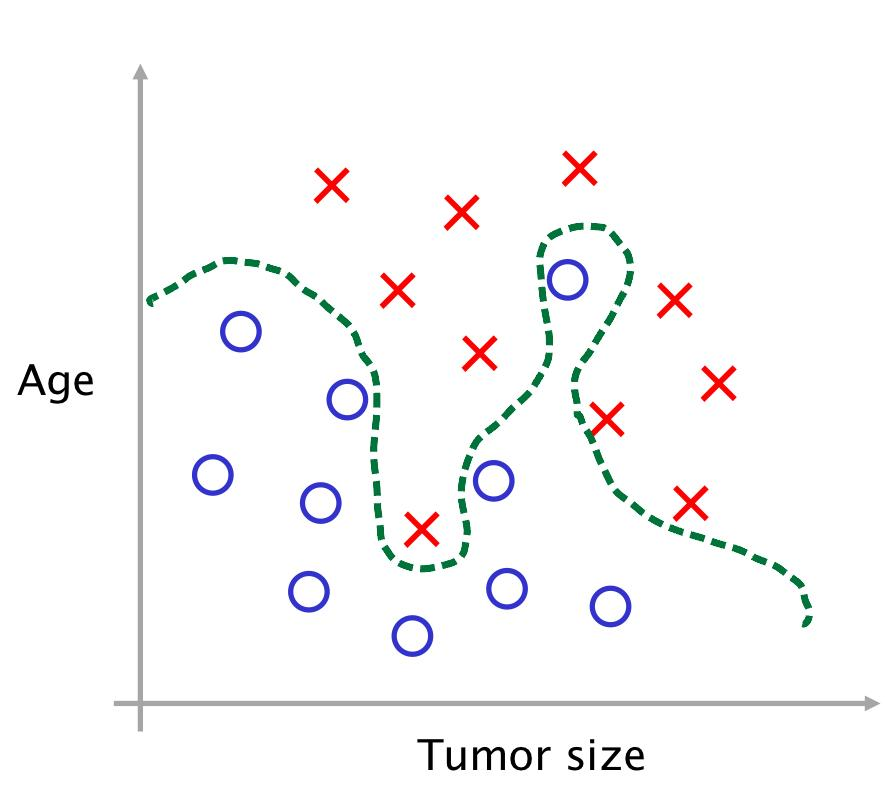
\includegraphics[scale=0.2]{img/overfit.jpeg}
    \caption{Example of overfitting}
\end{figure}

\noindent
Is this a good model for the given problem? NO! This model will have very bad \textit{performances of generalization} with new records to be classified, since it is too much related to the given dataset. In a colloquial way we say that: \textsf{The model has learnt the by heart the dataset}. A problem known as \textbf{overfitting}. \\
Finally, we can say that few features will result in a bad model, on the other hand also too much features will result in a bad model for another problem known as the \textbf{curse of dimensionality}.\footnote{
    In these case techniques of dimensionality reduction has to be employed.
}

\section{Unsupervided learning}
At the opposite of the \textit{supervised approach}, here patterns are learnt exclusively from unlabeled data. The most common example of such an approach is the \textbf{Clustering}.

\subsection{Clustering}
In this case several algorithms are employed to discover groups called \textbf{clusters} associated with objects which are similar in some sense. In general, very often distance-based measures are used to individuate the groups. One of the most famous clustering algorithm is the \textit{K-Mean}. The following figure is an example of bivariate clustered data. 

\begin{figure}[h]
    \centering
    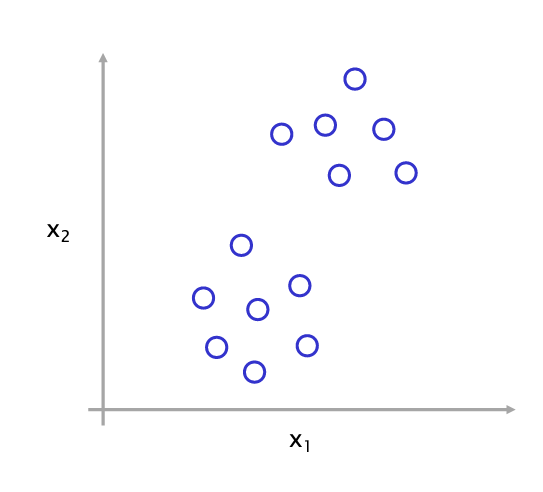
\includegraphics[scale=0.5]{img/clustering.png}
\end{figure}

Unsupervised techniques are used also in bioinformatics in manipulated \textit{DNA microarrays}, for gropuing together similar web pages, for analysis of astronomical data and so on.